\chapter{Periodic orbits in chaotic systems}
\label{chap:orbits}

%% CONTRIBUTION
\small \paragraph{Contributions} This chapter is largely based on the following publication\footnote{with the following author contributions.
Conceptualisation: MK, PVC, EAP. Data curation: MK. Formal Analysis: MK. Methodology: MK. Visualisation: MK. Writing – original draft:
MK. Writing – review and editing: MK, PVC, EAP, TNP. The contributions of Peter, Adam and Tim are highly appreciated.}

\vspace{\baselineskip}
\indent M Klöwer, PV Coveney, EA Paxton, and TN Palmer, 2021.
\emph{On periodic orbits in chaotic systems simulated at low precision}, in preparation.
\vspace{\baselineskip}
\normalsize

\section{Introduction}

Many natural systems exhibit chaotic dynamics.

\section{Methods}

Floating-point numbers are standardized following IEEE, 1985, 2008. Another number format used here are posits
(\cite{Gustafson2017a}, and section \ref{sec:posits}), which have a slightly higher precision within the powers of 2
around $\pm1$, yet a wide dynamic range at the cost of a gradually lower precision away from $\pm1$. While posits
have been proposed as a drop-in replacement for floats, they currently lack widely available hardware support.
Logarithmic fixed-point numbers have received little attention apart from research implementations on custom hardware
\citep{Johnson2020} and are described in section \ref{sec:logfixs} with our design choices in more detail.
Stochastic rounding has recently emerged as an alternative rounding mode to the widely used deterministic round-to-nearest
(section \ref{sec:roundnearest}, \cite{IEEE1985}), beneficial for scientific computing
\citep{Croci2020,Fasi2021,Hopkins2020,Paxton2021} and is described in section \ref{sec:stochastic_rounding}. An improved
pseudo random number generator for floats is presented in \ref{sec:randfloat} which is used for Monte Carlo-based
search for periodic orbits (section \ref{sec:orbit_search}). Especially for systems of several variables, the search for
periodic orbits becomes computationally very demanding and we outline our approach using distributed computing
in section \ref{sec:distributed_orbit_search}. The agreement between invariant measures is analysed with the
Wasserstein distance, which is briefly described in section \ref{sec:wasserstein}.

\subsection{An improved random number generator for uniformly distributed floats}
\label{sec:randfloat}

Conventional random number generation for a float $f$ from a uniform distribution $U(0,1)$
in $[0,1)$ uses the following technique: First, 10, 23, or 52 random bits (for Float16, Float32, or Float64, respectively)
from an unsigned integer are used to set the mantissa bits of floating-point one. This creates a floating-point
number that is uniformly distributed in $[1,2)$ as all float formats are uniformly distributed in that range. Second,
$1$ is subtracted to obtain a float in $[0,1)$, i.e. $f \sim U(1,2) - 1$. While this approach is fast, it is statistically
imperfect as the resulting distribution does not contain all floats in $[0,1)$ due to the rounding error introduced
by the subtraction. This technique only samples from every second float in $[\tfrac{1}{2},1)$, every fourth in
$[\tfrac{1}{4},\tfrac{1}{2})$ and so every $2n$-th float in $[2^{-n-1},2^{-n})$. Furthermore, the smallest positive
number that can be obtained is about $10^{-7}$ for Float32 and $10^{-16}$ for Float64. This is many orders of
magnitude larger than minpos, the smallest representable positive float, which is about $10^{-45}$, $10^{-324}$ for
Float32, Float64, respectively.

We therefore developed a statistically improved conversion from a random unsigned integer to a uniformly distributed
float in $[0,1)$. Counting the number of leading zeros $l$ of a random unsigned integer yields $l = 0$ at probability
$p = \tfrac{1}{2}$, $l=1$ at probability $p=\tfrac{1}{4}$ and $l = k$ at probability $p=2^{-k-1}$. These probabilities
correspond exactly to the share of power-2 exponents in the unit range $[0,1)$ for floats.
Consequently, we translate the number of leading zeros $l$  to the respective exponent bits and use the remaining
bits of the unsigned integers for the mantissa bits. The statistical flaws from the conventional conversion as presented
above are avoided, but for practical reasons the smallest float that can be sampled is about $10^{-20}$ for both Float32
and Float64. It is therefore practically impossible to sample a zero with this technique, just as the chance of obtaining a
zero in $[0,1)$ is effectively 0 for floats with 32 or 64 bit. For Float32, for example, we implement this technique as shown
in Listing \ref{lst:randfloat}, the implementations for Float16 and Float64 are similar. See our implementation in the Julia-package
\href{https://github.com/JuliaRandom/RandomNumbers.jl}{RandomNumbers.jl} for further details. The random number generation
for uniformly distributed floats is used throughout this study.

\begin{figure}[tbhp]
\begin{lstlisting}[language=JuliaLocal,label=lst:randfloat,caption={\textbf{An improved random number generator (RNG) for uniformly
distributed floats.} The Julia function \texttt{randfloat} takes \texttt{rng} as an argument for an RNG for 64-bit unsigned integers \texttt{UInt64}.
\texttt{\%} is the remainder after division, for unsigned integers effectively converting between unsigned integers by adding leading
zeros or discarding leading bits. \texttt{?} indicates a one-line if-clause. \texttt{\&} is the bitwise logical and-operation. \texttt{$\vert$}
is the bitwise logical or-operation.}]
function randfloat(rng::Random.AbstractRNG,::Type{Float32})

    # 64 random bits with generator rng
    ui = rand(rng,UInt64)

    # count leading zeros of random UInt64
    lz = leading_zeros(ui)

    # then convert leading zeros to exponent bits of Float32
    # e.g. 01111110, and bitshift to the right position via <<23
    e = ((126 - lz) % UInt32) << 23

    # reuse the last bits of ui for the 23 mantissa bits
    # unless the leading zeros reach into those for lz > 40
    ui = lz > 40 ? rand(rng,UInt64) : ui

    # ui % UInt32 drops the first 32 bits
    # & 0x007f_ffff sets non-mantissa bits to 0
    # e | then combines exponent and mantissa
    # and reinterpret the UInt32 as Float32
    return reinterpret(Float32,e | ((ui % UInt32) & 0x007f_ffff))
end
\end{lstlisting}
\end{figure}

\subsection{Monte Carlo orbit search}
\label{sec:orbit_search}

The state of a deterministic dynamical system is entirely determined by $X = (X_1,X_2,...,X_N)$, the vector of all its $N$
prognostic variables at a given time step $t$. We define a periodic orbit when the state vector $X^{t_0}$ at time step $t_0$
reoccurs at a later time step $t_1 > t_0$
\begin{equation}
	X^{t_0} = X^{t_1}
	\label{eq:periodic_orbit}
\end{equation}
Bitwise equality is hereby required with an exception for floats where $-0 = 0$, which arithmetically does not impact on the
dynamical system. While $\tfrac{1}{-0} = -\infty \neq \infty = \tfrac{1}{0}$ in float arithmetic, we consider finite solutions only.
The bitwise periodicity is in contrast to other studies investigating quasi-periodic orbits \citep{Urminsky2010,Yalniz2021},
which usually only require $X^{t_0}, X^{t_1}$ to be close, but not bitwise identical.

The invariant measure of a chaotic system describes its attractor independent of the initial conditions. A deterministic chaotic
system simulated with finite-precision arithmetic (also deterministic as opposed to stochastic rounding, for example) will converge
to one of the periodic orbits for any initial condition. Based on all periodic orbits we can compute the invariant measure through
a weighted average by the orbits’ respective basins of attraction, i.e. the fraction of initial conditions that end up on a given
periodic orbit. To find \emph{all} periodic orbits in a deterministic dynamical system, all possible initial conditions have to be
integrated and checked for periodicity. For a 1-variable system with $X \in [0,1)$ (such as the Bernoulli map, see section
\ref{sec:revisit_bernoulli}) simulated with Float32 there are 1,065,353,216 initial conditions. For any larger system or
higher precision number format it becomes computationally virtually impossible to consider all initial conditions. We therefore
use a Monte Carlo-based random sampling of the initial conditions to find a subset of all orbits. The orbits found are statistically
expected to be those with the largest basins of attraction, and a robust estimate of their size is obtained for a sufficiently large
sample of initial conditions. This procedure is explained in the following.

\begin{figure}[tbhp]
	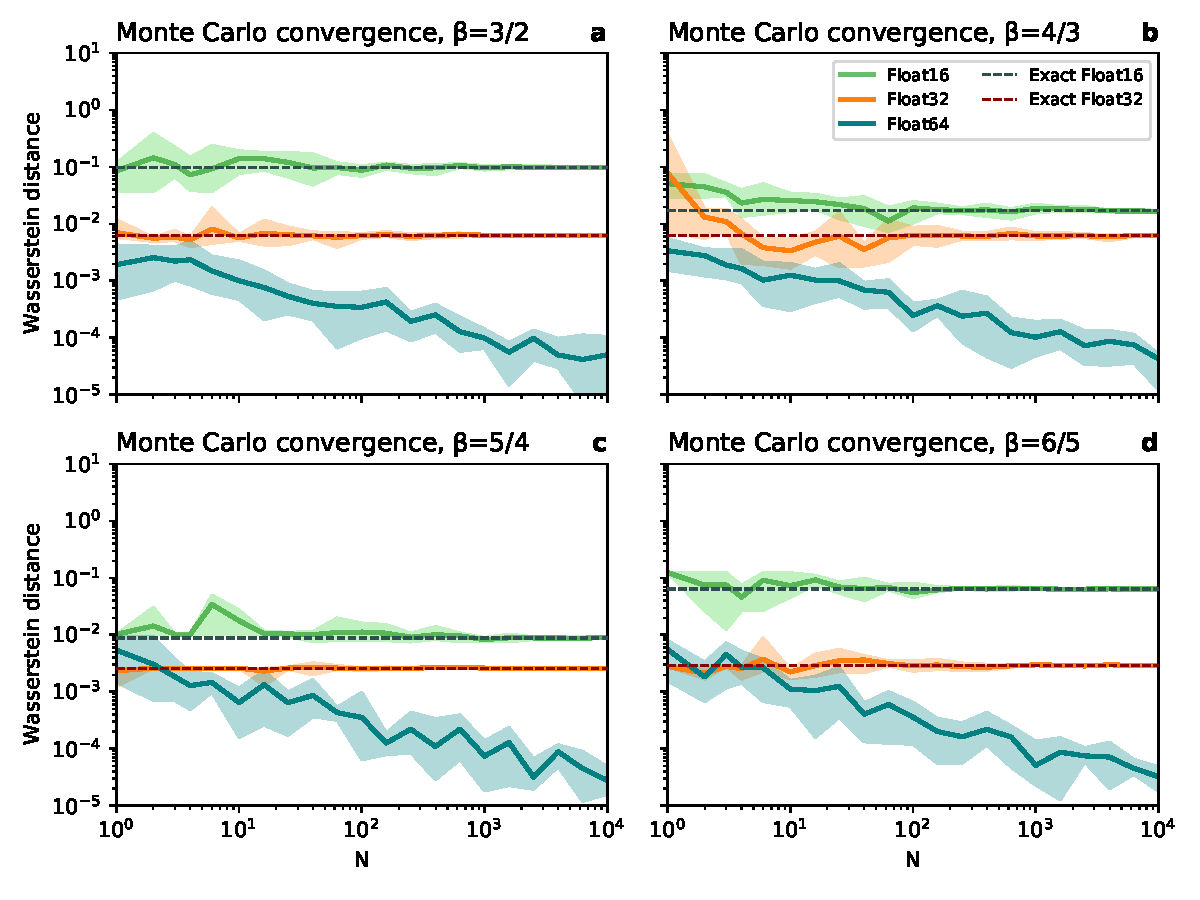
\includegraphics[width=1\textwidth]{Figures/orbits/convergence.pdf}
	\caption{\textbf{Convergence of the Monte Carlo sampling to estimate invariant measures.}
	The agreement between the analytical and simulated invariant measures (Figure \ref{fig:orbits_inv_measures})
	from $N$ random initial conditions uniformly distributed in $[0,1)$ are assessed with the Wasserstein distance
	(section \ref{sec:wasserstein}). About $N = 1000$ random initial conditions allow for a robust estimate of the
	invariant measure with Float16 and Float32, virtually identical with exact invariant measure obtained from
	computing all 15,360 Float16 and 1,065,353,216 Float32 numbers in $[0,1)$, respectively. The $\beta$ parameter
	of the generalised Bernoulli map is \textbf{a} $\beta = \tfrac{3}{2}$, \textbf{b} $\beta = \tfrac{4}{3}$,
	\textbf{c} $\beta = \tfrac{5}{4}$, and \textbf{d} $\beta = \tfrac{6}{5}$. Solid lines represent the mean and shading
	the min-max range.}
	\label{fig:orbits_convergence}
\end{figure}

For the generalised Bernoulli map, the random number generator from section \ref{sec:randfloat} is used to sample from all floats
in $[0,1)$ to obtain a representative subset of all initial conditions. While there is no guarantee that all orbits are found, those found
have the largest basin of attraction. While it is easily possible to miss a periodic orbit,
those missed have a very small basin of attraction and therefore a negligible contribution to the invariant measure. Estimating
the invariant measure from these orbits is therefore also expected to be an unbiased approximation that converges to the
exact invariant measure. The exact invariant measure, on the other hand, is obtained by finding \emph{all} simulated orbits
and their exact basins of attraction rather than using a random set of initial conditions. We verify this methodology for
Float16 and Float32, where the exact invariant measure can be calculated in Figure \ref{fig:orbits_convergence}. While we cannot
find all orbits with Float64, the Monte Carlo-based invariant measure converges to the analytical invariant measure and is
for the same sample size a better approximation than using Float16 or Float32. Despite the high precision, a Float64 simulation
of the generalised Bernoulli map still substantially degrades some properties of the analytical system: The topological entropy,
measuring how trajectories diverge onto distinct orbits, is positive in the analytical system, representing chaotic solutions.
However, even with the high precision of Float64 the topological entropy is negative, as trajectories eventually converge
onto periodic orbits.

For the Lorenz 1996 system, the space of all possible initial conditions is much larger than the space the attractor occupies.
It is therefore more efficient to only choose initial conditions randomly that are already part of, or at least close to the attractor.
Basin of attraction is here therefore the relative share of the initial conditions from the attractor that end up on a given orbit,
and not from all possible initial conditions. To obtain an initial condition for the Lorenz 1996 system, one first starts a high-precision
simulation from a given initial condition including a small stochastic perturbation (see section \ref{sec:orbits_lorenz96} for more
details). After disregarding a spin-up the information of the chosen initial condition is removed and the stochastic perturbation
grows into a fully independent random initial condition. Converting a random time step from a high-precision simulation into
the given number format then yields a point that is either on or close to the low-precision attractor.

\subsection{Efficient orbit search with distributed computing}
\label{sec:distributed_orbit_search}

\subsection{Wasserstein distance}
\label{sec:wasserstein}

The invariant measure of a chaotic dynamical system is estimated with histogram binning. To assess the agreement
of two histograms representing invariant measures (either simulated or analytical) we use the Wasserstein distance,
a metric that derives from the theory of optimal transport, with an $L^1$ cost. The Wasserstein distance $W_1(\mu,\nu)$
is defined as the least cost at which one can transport all probability mass from histogram $\mu$ to another histogram $\nu$,
where the cost to move mass $m$ from a bin at location $x$ to a bin at location $y$ is $m \vert x-y \vert$ \citep{Paxton2021,Villani2003}.
This gives a non-parametric method to compare probability distributions which accounts for both differences in the probabilities
of events as well as their separations in the underlying space, so that closeness in Wasserstein distance truly corresponds
to a natural notion of closeness between probability distributions \citep[Thm 7.12]{Villani2003}.

\section{Revisiting the generalised Bernoulli map}
\label{sec:revisit_bernoulli}

The generalised Bernoulli map \citep{Parry1960} is a 1-variable chaotic system starting with $x_0 \in [0,1)$
at time iteration $i=0$ with the parameter $\beta > 1$ defined as
\begin{equation}
	x_{i+1} = f_\beta(x_i) = \beta x_i \mod 1
	\label{eq:bernoulli}
\end{equation}
The modulo-operator $\mod$ satisfies that $x \in [0,1)$ in all future iterations. Simulating this system was found to not represent
well the periodic orbit spectrum \citep{Boghosian2019}, which is closely related to the simulated invariant measure. For the
generalised Bernoulli map the analytical invariant measure is known \citep{Hofbauer1978}
\begin{equation}
	h_\beta(x) = C\sum_{j=0}^\infty \beta^{-j} \theta(1_j - x)
	\label{eq:hofbauer}
\end{equation}
The heaviside function is $\theta$ and $1_j$ is the $j$-th iteration of the Bernoulli map starting from $x_0 = 1$, i.e. $1_j = f_\beta^j(1)$.
The normalization constant is chosen as $C=1$, but for the calculation of Wasserstein distances renormalization is applied so that
$C\int_0^1h_\beta(x) \mathrm{d}x = 1$, which ensures that $Ch_\beta(x)$ is a probability density function. To better visualise the
invariant measure for varying $\beta$ we introduce a normalisation $h_\beta^*(x) = \tfrac{h_\beta(x)}{\max(h_\beta(x))}$, which is always
in $[0,1]$ and can be applied to the analytical invariant measure as well as simulated ones.

We are revisiting the generalised Bernoulli map with various number formats and rounding modes to understand better the previously
suggested pathology \citep{Boghosian2019} as a function of arithmetic precision. While simulating the Bernoulli map numerically with
a given number format, we perform both the multiplication and the subtraction in Eq. \ref{eq:bernoulli} with that format and avoid any
conversion between number formats. This is in contrast to \cite{Boghosian2019}, whose implementation converts $x_i$ to Float64
before multiplication with $\beta$ (as Float64) and possible subtraction with 1 (as Float64) in the modulo. In summary, 
$x_{i+1} = \op{Float32}(\beta * \op{Float64}(x_i) \mod 1)$. While some hardware allows for fused multiply-add operations without
intermediate rounding error, similar to the conversion to Float64 here, the fused conditional subtraction in the modulo is generally not
supported on hardware.

\begin{figure}[tbhp]
	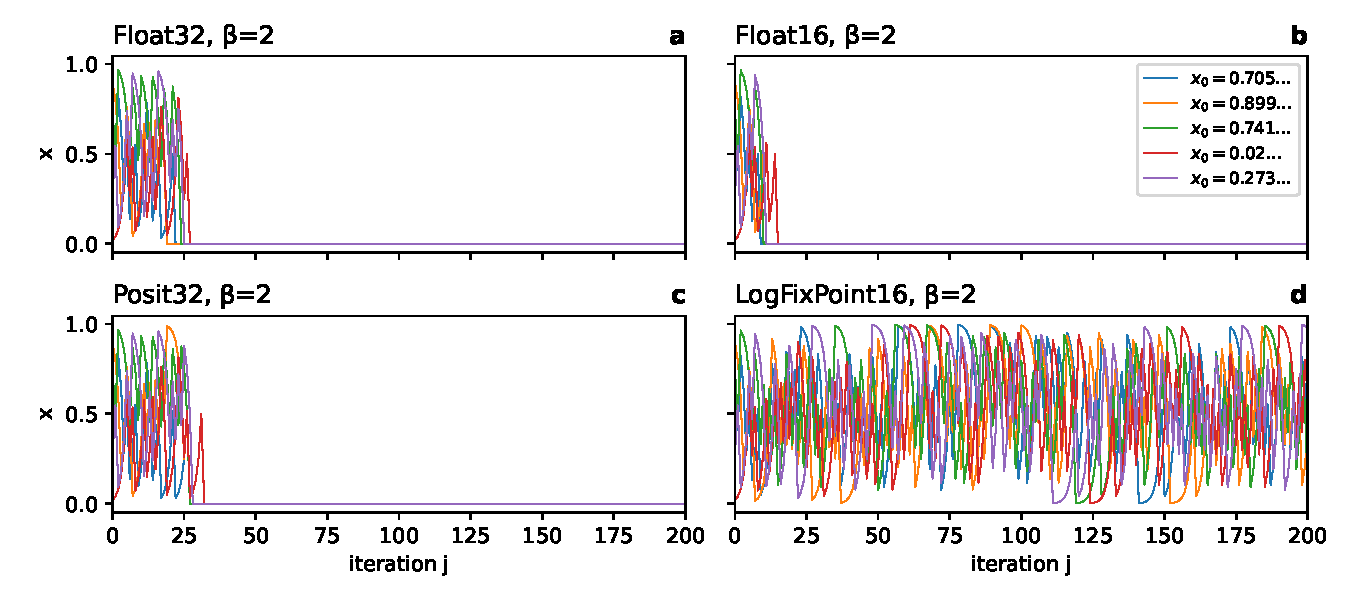
\includegraphics[width=1\textwidth]{Figures/orbits/beta2.pdf}
	\caption{\textbf{The Bernoulli map simulated with different number formats. a}
	Float32, \textbf{b} Float16, \textbf{c} Posit32, and \textbf{d} LogFixPoint16. The arithmetic operations in the
	Bernoulli map do not introduce rounding errors in \textbf{a}-\textbf{c}, only the initial conditions are subject
	to rounding, causing the attractor to collapse after a few iterations. However, the subtraction in the Bernoulli
	map causes rounding errors with logfix arithmetic in \textbf{d} that prevent the stalling at 0 from \textbf{a}-\textbf{c}.}
	\label{fig:orbits_beta2}
\end{figure}

\subsection{The special $\beta = 2$ case}
\label{sec:orbits_beta2}

\cite{Boghosian2019} highlight that the Bernoulli map with $\beta = 2$, and similarly for every even integer, will collapse to $x=0$
after $n$ iterations with any float format at arbitrary high precision, where $n$ is smaller than the number of bits in the format.
The multiplication with $\beta = 2$ acts as a bitshift in base-2 format towards more significant bits, pushing zero bits in the mantissa
and subsequently also into the exponent, eventually setting $x$ to 0 (Figure \ref{fig:orbits_beta2}a, b and c). This phenomenon occurs
as the Bernoulli map with $beta=2$ (and similarly for larger even integers) does not introduce any arithmetic rounding error: Both the
multiplication with $\beta$ and subtraction with 1 are exact with floats (and also with posits) in $[1,2)$. The multiplication with $\beta=2$
is exact as the base-2 exponent is simply increased by 1. The subtraction with 1 is exact as every finite positive float (subnormals excluded)
or posit can be written as $2^e(1+f)$ (see Eq. \ref{eq:float}) for some integer exponent $e$ and a sum $f \in [0,1)$ of powers of two
with negative exponents. Constraining the range to $[1,2)$, where the subtraction is applied, yields $e=0$ and so the subtraction of $1+f$
with 1 is $f$, again a sum of powers of two, which is exactly representable with floats or posits.

The only occurring rounding error is in the initial conditions. While a randomly chosen $x \in [0,1)$ will have infinitely many non-zero
mantissa bits at infinite precision, at finite precision those beyond the resolved mantissa bits will be rounded to 0. Therefore, the least
significant mantissa bit remains 0 after each iteration of the Bernoulli map while the same 0 bit from the previous iteration is further
shifted in. While this behaviour holds for floats and posits, it does not occur with logarithmic fixed-point numbers (logfixs). All multiplications
are exact with logfixs (unless under or overflows occur, see section \ref{sec:logfixs}), but in contrast to floats and posits a rounding error
occurs in the subtraction, with the possibility of setting the least significant mantissa bit to 1. On the next multiplication with
$\beta=2$ this 1-bit is shifted further in, hence, the rounding error is effective at preventing a collapse of the attractor
(Figure \ref{fig:orbits_beta2}d). The Bernoulli map with $\beta=2$ and simulated with floats or posits is therefore special, as it is a
chaotic system that does not involve any arithmetic rounding errors beyond the rounding of the initial conditions. However, the
simulation of most other system, including the generalised Bernoulli map with $1<\beta<2$, involves rounding errors with any 
finite precision number format.

\begin{figure}[tbhp]
	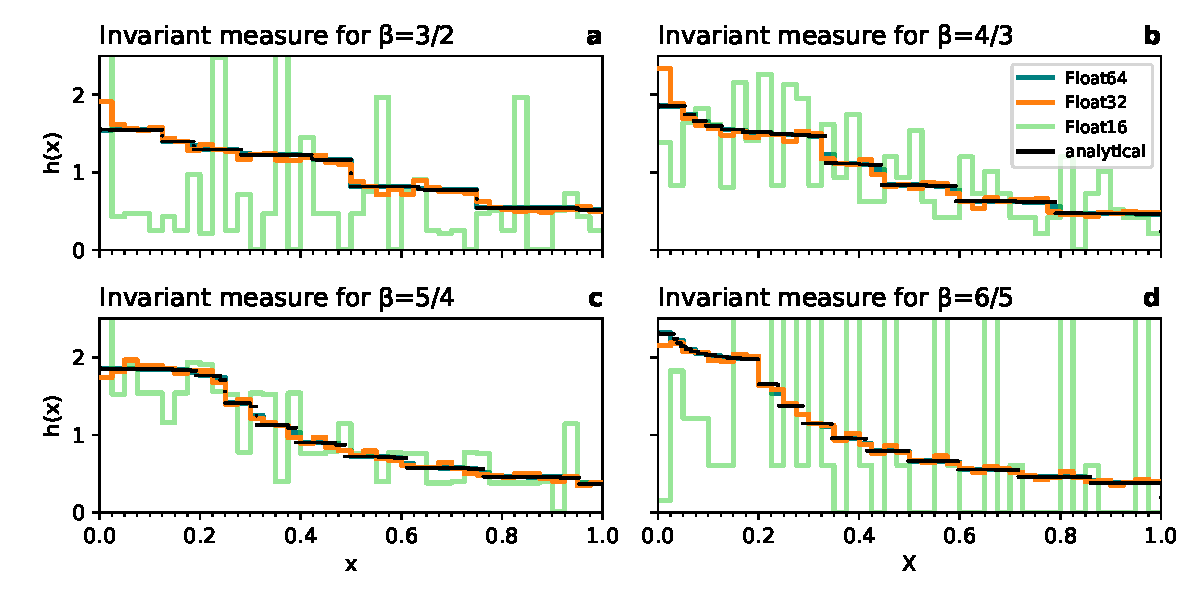
\includegraphics[width=1\textwidth]{Figures/orbits/inv_measures.pdf}
	\caption{\textbf{The invariant measure of the generalised Bernoulli map.}
	The generalised Bernoulli map is simulated with parameter \textbf{a} $\beta = \tfrac{3}{2}$,
	\textbf{b} $\beta = \tfrac{4}{3}$, \textbf{c} $\beta = \tfrac{5}{4}$, \textbf{d} $\beta = \tfrac{6}{5}$ and
	calculated with different number formats Float64, Float32 and Float16. The invariant measures of
	Float16 and Float32 are obtained from periodic orbits found by starting from 10,000 initial conditions
	$x_0 \in [0,1)$ chosen from a random uniform distribution. For Float64, long integrations (10,000 iterations,
	disregarding a spin-up of 5,000 iterations) of the Bernoulli map are used instead.
	Histograms use the bin width 0.025. The analytical invariant measure is not binned,
	which accounts for the discrepancy to Float64.}
	\label{fig:orbits_inv_measures}
\end{figure}

\subsection{Bifurcation of the invariant measure}
\label{sec:bifurcation}

Given that the analytical invariant measure is known for the generalised Bernoulli map (Eq. \ref{eq:bernoulli}), we can assess
the representation of such a system with various number formats at different levels of precision. \cite{Boghosian2019} conclude
that the invariant measure with Float32 is an inaccurate approximation of the analytical invariant measure. This difference is even
more pronounced with Float16 arithmetic (Figure \ref{fig:orbits_inv_measures}), however, with Float64 the invariant measure is
comparably accurate. The question therefore arises whether the discrepancy of the invariant measures vanishes with higher precision,
or whether a pathology persists at any precision level for some $\beta < 2$.

The analytical invariant measure of the generalised Bernoulli map consists of many step functions taking values on a discrete set
of points (Fig. \ref{fig:orbits_inv_measures}), which bifurcate with increasing (Fig. \ref{fig:orbits_bifurcation}a). These \emph{quantization levels}
cannot be exactly represented with Float16 or Float32 arithmetic (Fig. \ref{fig:orbits_inv_measures}),, such that their bifurcation is visually
blurred (Fig. \ref{fig:orbits_bifurcation}c). However, the visually sharp representation of this bifurcation of the quantization levels with Float64
indicates a much more accurate approximation to the analytical invariant measure. Due to the higher precision of 32-bit posit arithmetic
(Posit32) around $\pm1$, the bifurcation is slightly improved with Posit32 over Float32 (Fig. \ref{fig:orbits_bifurcation}d). Given the
inaccurate representation of the invariant measure with Float16 (Fig. \ref{fig:orbits_inv_measures}), its bifurcation has little resemblance
to the analytical bifurcation (Fig. \ref{fig:orbits_bifurcation}f).

\begin{figure}[tbhp]
	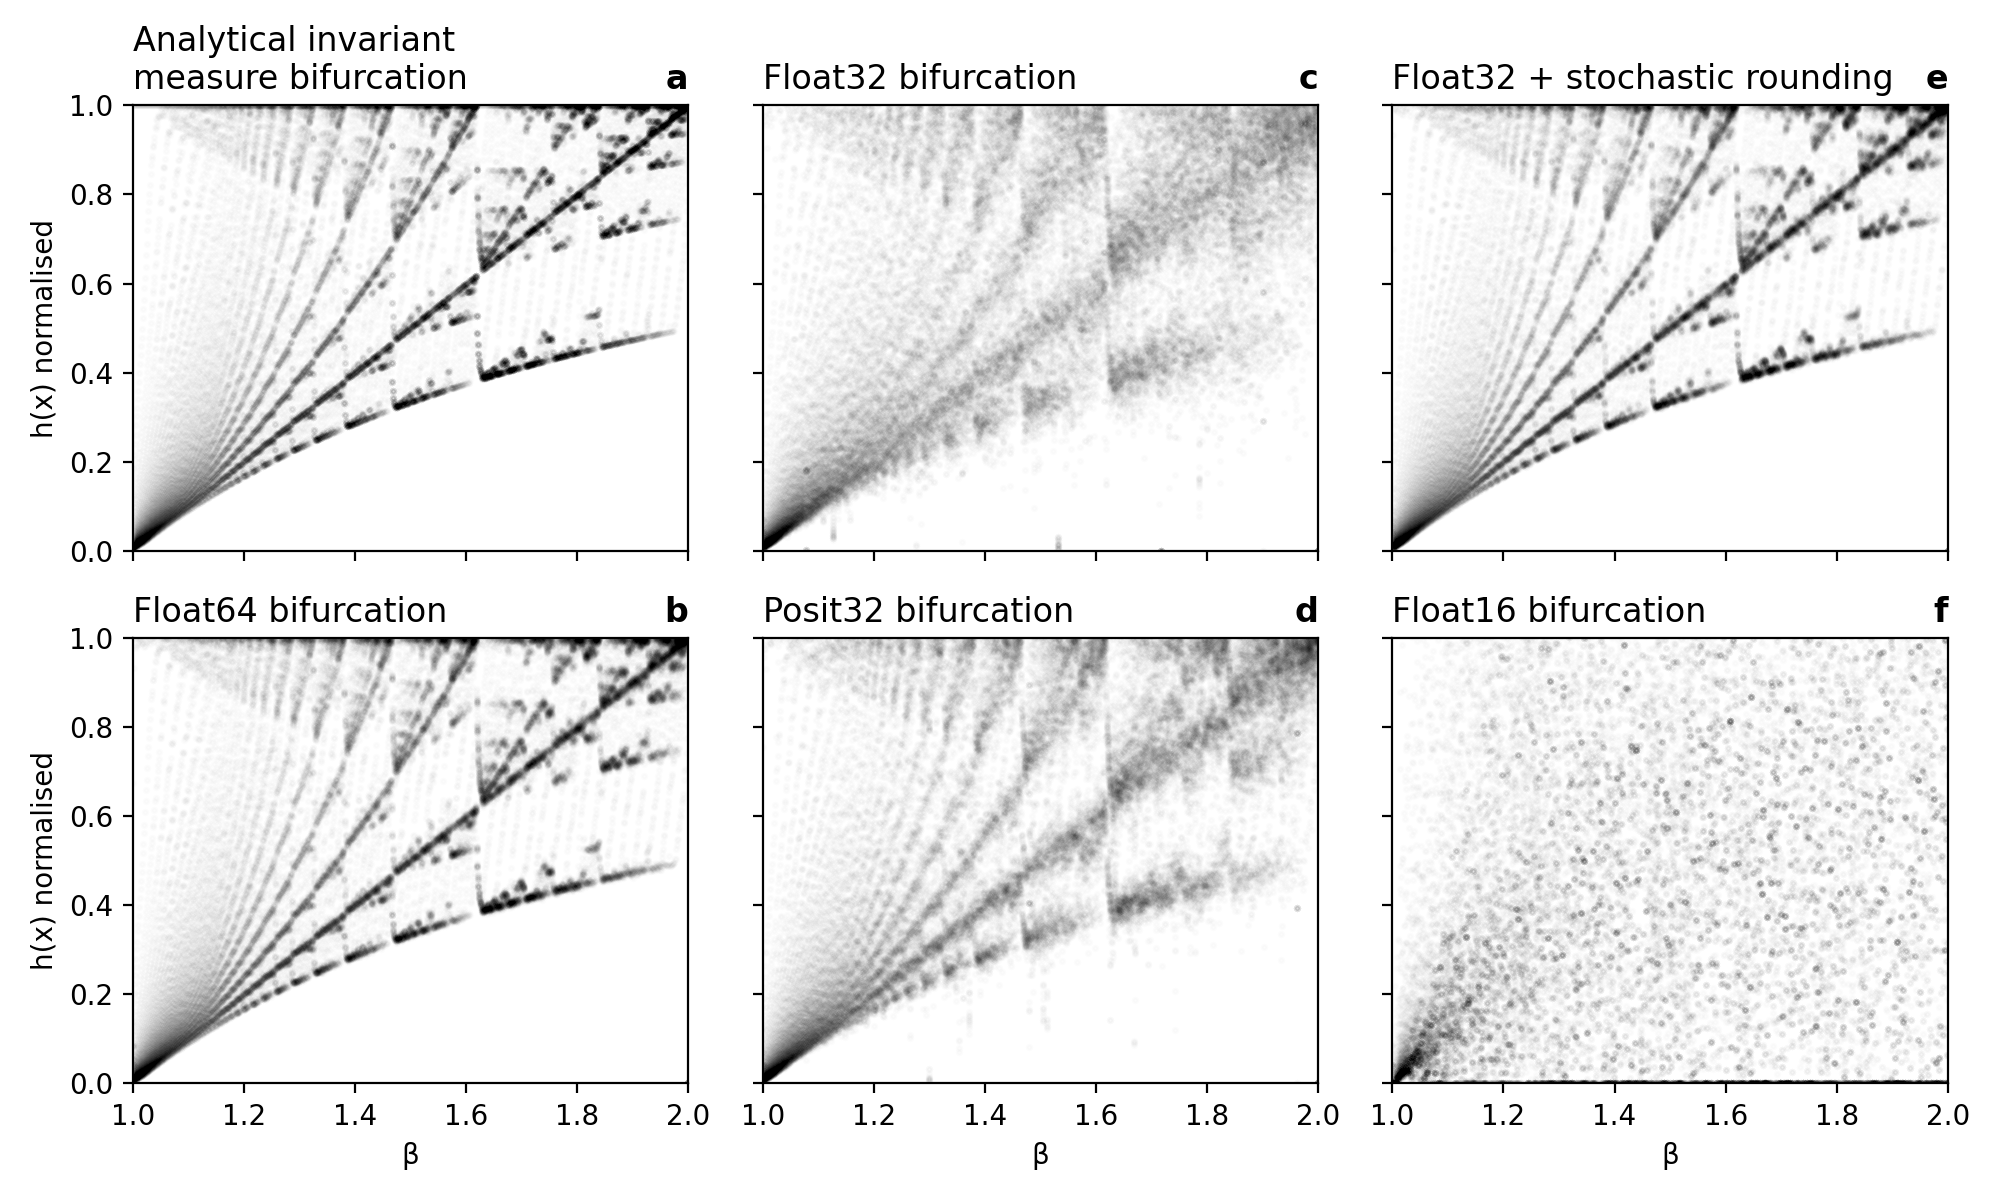
\includegraphics[width=1\textwidth]{Figures/orbits/bifurcation.png}
	\caption{\textbf{Bifurcation of the quantization levels corresponding to the invariant measures in
	the generalised Bernoulli map as simulated with various number formats. a}
	Analytical bifurcation $h_\beta(x)$ from the exact invariant measure, normalised by $\max(h_\beta(x))$,
	compared to the invariant measure by simulating the Bernoulli map with \textbf{b} Float64, \textbf{c} Float32,
	\textbf{d} Posit32, \textbf{e} Float32 and stochastic rounding, and \textbf{f} Float16.}
	\label{fig:orbits_bifurcation}
\end{figure}

\subsection{Effects of stochastic rounding}
\label{sec:orbits_stochastic_rounding}

Augmenting Float32 with stochastic rounding considerably improves the bifurcation of the invariant measure (Fig. \ref{fig:orbits_bifurcation}e)
and makes it virtually indistinguishable from Float64 or the analytic bifurcation. However, stochastic rounding does not decrease the rounding
error accumulated over many iterations in a forecast (Figure \ref{fig:orbits_error_growth}), such that the effective precision is not increased
over deterministic rounding. But introducing stochasticity prevents the convergence onto short periodic orbits, which are otherwise present
with deterministic rounding \citep{Boghosian2019}. Previously inaccessible regions of the attractor can be reached with stochastic rounding
as the simulation is frequently pushed off any periodic orbit. While periodic orbits are not fully removed from solutions due to the use of
pseudo random number generators (PRNG) that are themselves periodic, the periods of PRNGs are usually so long that effectively any
periodicity is avoided. The period length of the conventional Mersenne Twister \citep{Matsumoto1998} is $2^{19937}-1$ and still sufficiently
long with $2^{128} - 1$ for the faster Xoroshiro128+ \citep{Blackman2019} PRNG that is used in StochasticRounding.jl.

\begin{figure}[tbhp]
	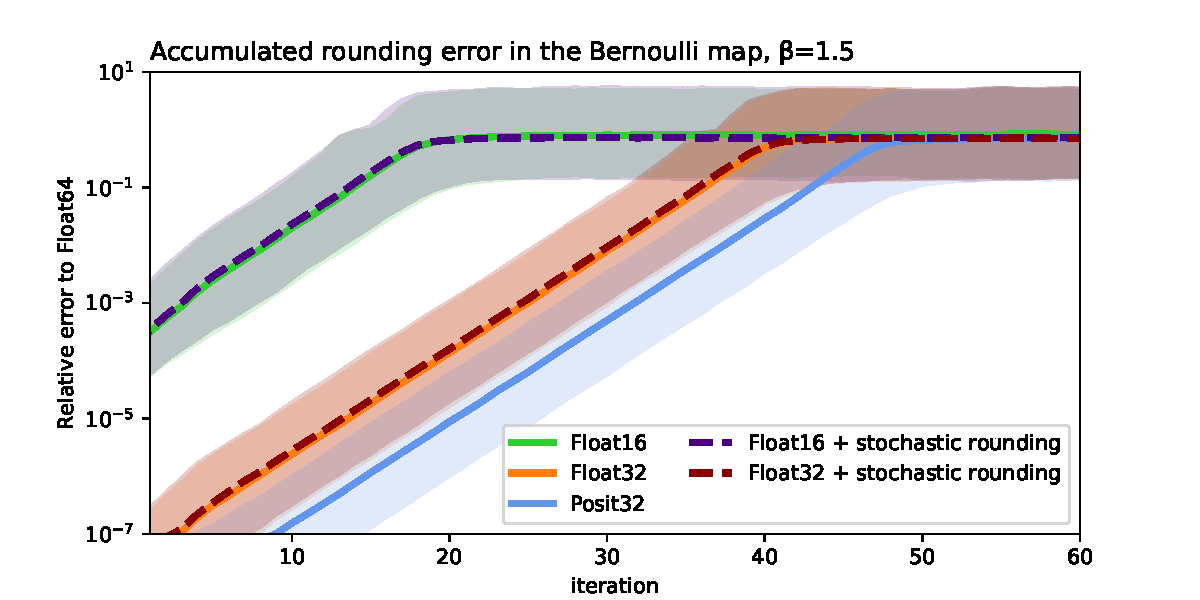
\includegraphics[width=1\textwidth]{Figures/orbits/error_growth.pdf}
	\caption{\textbf{Accumulated rounding error in the Bernoulli map.}
	Starting from 10,000 random initial conditions, the accumulated rounding error is the relative error of the
	given number format relative to a Float64 integration. Solid lines represent median errors across all
	initial conditions, shading the interdecile range. Other choices for the parameter $\beta$ of the generalised
	Bernoulli map yield a similar comparison between the number formats, but decreasing $\beta$ towards 1
	decreases the error growth for all formats similarly.}
	\label{fig:orbits_error_growth}
\end{figure}

The agreement of the analytical and simulated invariant measures is quantified with the Wasserstein distance (section \ref{sec:wasserstein}).
For $\beta=2$ the analytical invariant measure is the uniform distribution $U(0,1)$, whereas all float and posit formats for both deterministic
and stochastic rounding simulate a collapse of the attractor to zero such that the invariant measure is the Dirac delta distribution
(Fig \ref{fig:orbits_beta2}). The Wasserstein distance is in all these cases $W_1 = 0.5$ and does not decrease, i.e. improve, with precision.
However, as previously mentioned, the rounding errors from logfixs prevent a collapse such that for LogFixPoint16 the invariant measure is
much better approximated, with $W_1 = 0.05$.

\begin{figure}[tbhp]
	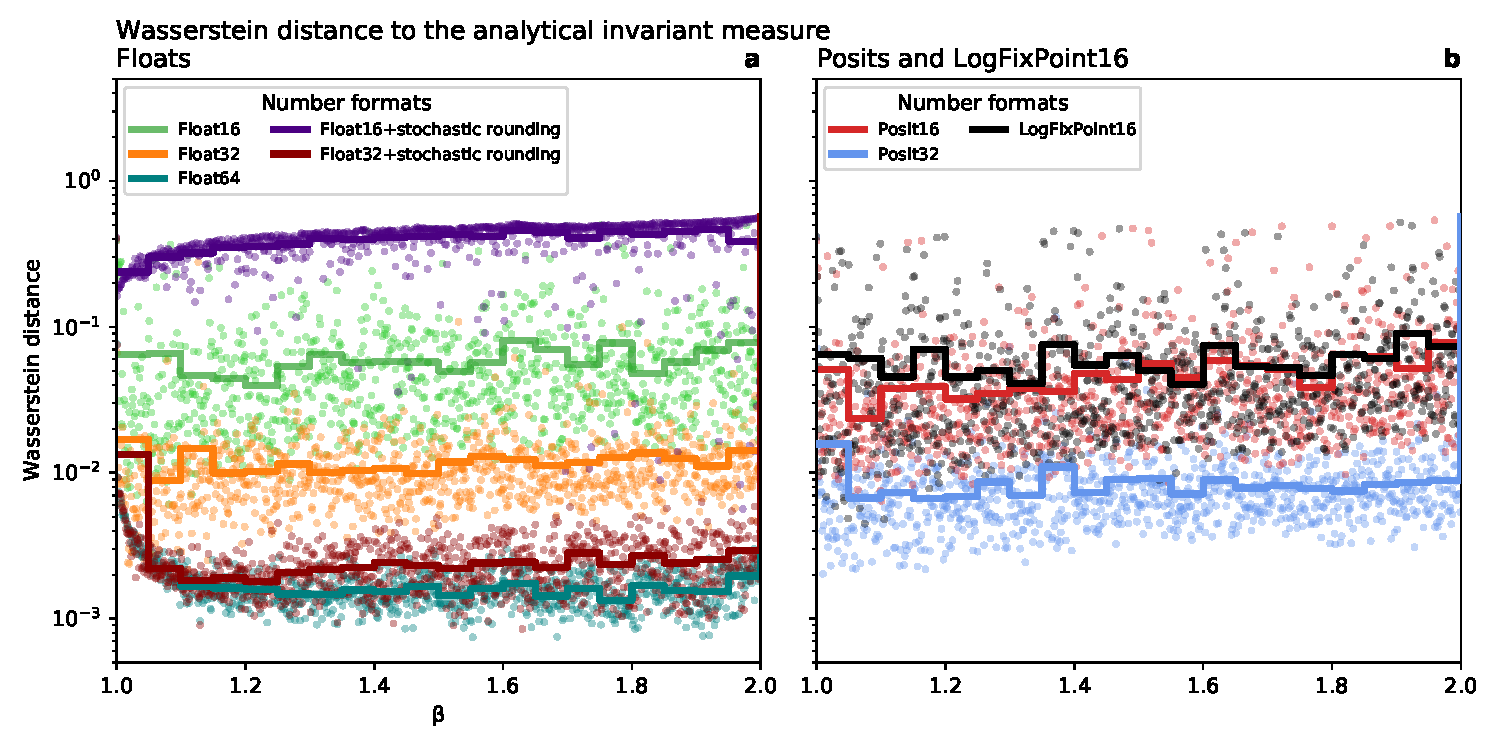
\includegraphics[width=1\textwidth]{Figures/orbits/wasserstein.pdf}
	\caption{\textbf{Agreement between the simulated and analytical invariant measures in the generalised
	Bernoulli map.} For all values except $\beta = 2$ a high precision number format yields a better agreement
	with the analytical Bernoulli map. Simulations using \textbf{a} Floats with and without stochastic rounding, 
	\textbf{b} Posits and LogFixPoint16. The Wasserstein distances are calculated for the invariant measures
	obtained from 1000 simulations for every value of $\beta$. Scatter points denote individual Wasserstein
	distances, solid lines indicate averages across a range of  as indicated by steps.}
	\label{fig:orbits_wasserstein}
\end{figure}

For $1<\beta<2$  the Wasserstein distance is always reduced going to higher precision, supporting the inference that only the case $\beta=2$
(and other even integers) presents a pathology where higher precision does not improve the simulated invariant measure arising from the
generalised Bernoulli map (Fig. \ref{fig:orbits_wasserstein}). The Wasserstein distances of Float32 with stochastic rounding are similarly low
to Float64, but Float64 yields slightly lower distances in most cases.

However, using stochastic rounding with Float16 is worse than deterministic rounding as here the stochasticity makes it possible that the
invariant measure of the generalised Bernoulli map collapses to 0, which is a fixed point (Figure \ref{fig:orbits_stochastic_collapse}).
While for Float32 the probability of such an occurrence is low and is not observed here, with Float16 most simulations collapse within
a few thousand iterations transforming their invariant measures into Dirac distributions. Whether this problem generalises to other
systems is questionable. We suspect that this is a feature of low dimensional dynamics, and would not arise in more physical,
higher dimensional systems, where the chance of a stochastic perturbation moving one onto a fixed point becomes vanishingly
small even at very low precision. Other natural systems do not have fixed points due to time-dependent forcing. The posit format
is slightly better than floats at both 16 and 32 bit, as expected from the slightly higher precision.

\begin{figure}[tbhp]
	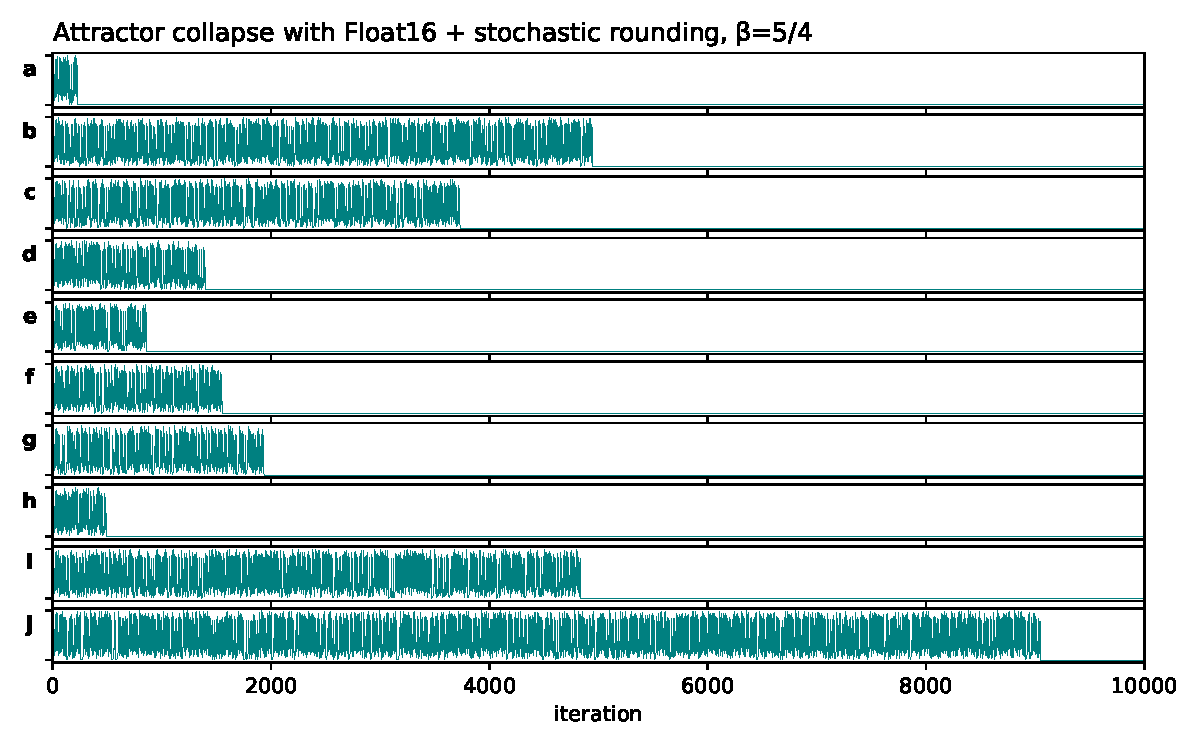
\includegraphics[width=1\textwidth]{Figures/orbits/attractor_collapse.pdf}
	\caption{\textbf{Attractor collapse of the generalised Bernoulli map with Float16 and stochastic roudning. a}-\textbf{j}
	Simulation of the Bernoulli starting from identical initial conditions and $\beta = 5/4$. Only the the
	state of the random number generator for stochastic rounding differs between \textbf{a}-\textbf{j}. After 10,000 iterations
	all simulations \textbf{a}-\textbf{j} stalled at the fixed-point 0 of the analytical attractor. The y-axes denote the value of
	$x_i$ in [0,1].}
	\label{fig:orbits_stochastic_collapse}
\end{figure}

\section{Orbits in the Lorenz 1996 system}
\label{sec:orbits_lorenz96}

In contrast to the 1-variable generalised Bernoulli map, most continuous natural systems are simulated with as many variables
as computationally affordable. Weather forecast and climate models often use more than 10 million independent variables that
result from a discretisation of naturally continuous variables on the globe. While short periodic orbits in low precision are problematic
in the simulation of few-variable systems as discussed in the previous section, this section tests the hypothesis that large systems are
unaffected for all practical purposes.

\subsection{The Lorenz 1996 system}
\label{sec:lorenz96}

To investigate the dependence of periodic orbits on the number of variables in the system we consider the chaotic Lorenz 1996 system
\citep{Hatfield2017, Lorenz1998}. With $N$ variables $X_i,i=1,...,N$ the Lorenz 1996 system is a system of coupled ordinary differential
equations

\begin{equation}
	\frac{\mathrm{d}X_i}{\mathrm{d}t} = (X_{i+1} - X_{i-2})X_{i-1} - X_i + F
	\label{eq:lorenz96}
\end{equation}

in a 1-dimensional spatial domain with periodic boundary conditions, $X_{N+1} = X_1$ etc. The term $(X_{i+1} - X_{i-2})X_{i-1}$
implements nonlinear advection and drag is represented with the relaxation term $-X_i$. The forcing $F$ is the single parameter
in the Lorenz 1996 system fixed at the common default $F=8$ which produces chaotic solutions. The forcing is steady in time and
constant in space. The system exhibits dynamics of nonlinear wave-wave interactions (Fig. \ref{fig:orbits_hovmoeller}), which are
reasonably independent of the number of variables (Figure \ref{fig:orbits_hovmoeller}b). The system can be integrated with as little
as $N=4$ variables without an obvious degradation of the simulated dynamics.

\begin{figure}[tbhp]
	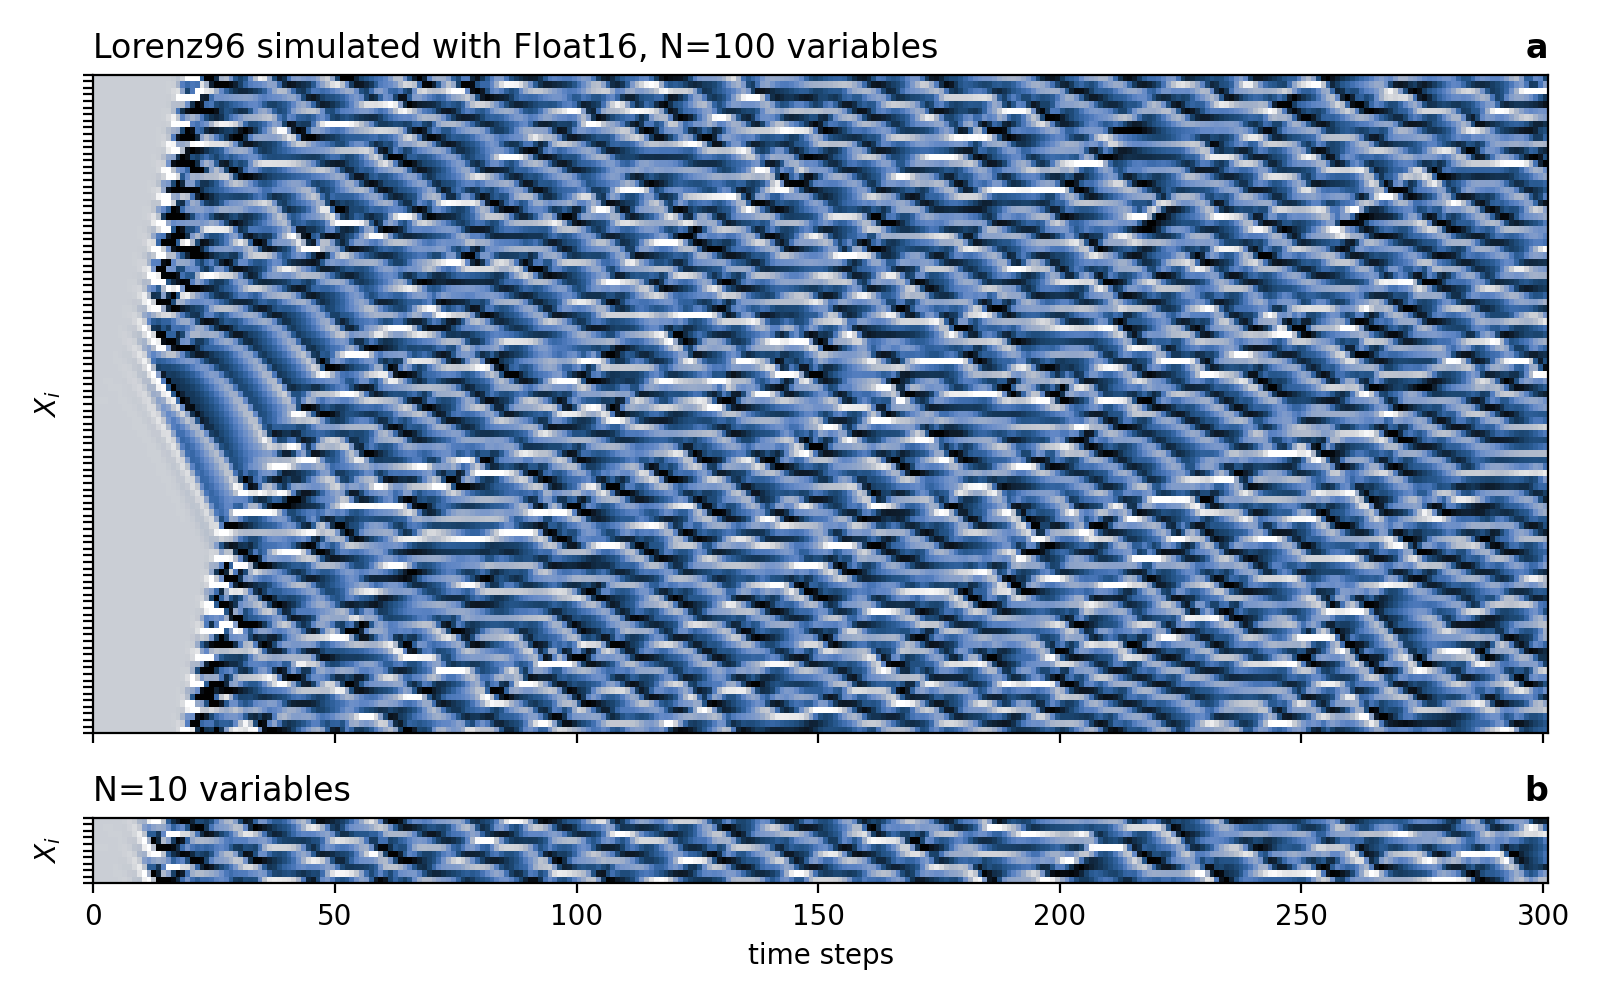
\includegraphics[width=1\textwidth]{Figures/orbits/hovmoeller.png}
	\caption{\textbf{The Lorenz 1996 system simulated with Float16 arithmetic. a}
	$100$ variables are used, starting from equilibrium with a small perturbation in $X_{50}$, and
	\textbf{b} $10$ variables starting with a small perturbation in $X_5$. Rectangles visible in shading
	represent individual variables and time step.}
	\label{fig:orbits_hovmoeller}
\end{figure}

The initial conditions are in equilibrium $X_i = F, \forall i i \neq j$ with only a single variable which is slightly perturbed, 
$X_j = F + 0.005 + 0.01\epsilon$ with $\epsilon \sim U(0,1)$, drawn from a random uniform distribution in $[0,1)$.
Due to the periodic boundary conditions, the system is spatially invariant once the information from the initial conditions
is removed through the chaotic dynamical evolution, after some several hundred time steps (Figure \ref{fig:orbits_hovmoeller}a).
The invariant measure $\mu$ of one variable $X_i$ is therefore identical to that of any other, $\mu(X_i) = \mu(X_j), \forall i,j$,
as will be further discussed below.

The Lorenz 1996 system is discretized in time using the 4-th order Runge-Kutta scheme \citep{Butcher2008} with a time
step of $\Delta t = 0.01$. At this temporal resolution the system can also be integrated using a low-precision number format
such as Float16 (Figure \ref{fig:orbits_hovmoeller}). For more details and a software implementation see Lorenz96.jl (Klöwer, 2019/2021).

\subsection{Longer orbits with more variables}

Using $N=4$ variables in the Lorenz 1996 system simulated with Float16, the longest periodic orbit we find is 6756 time steps long
(Figure \ref{fig:L96_orbits}). The basin of attraction is about 0.82, meaning that more than 80\% of the randomly chosen initial
conditions converge onto this orbit. Increasing the number of variables to $N=5$, the longest periodic orbit found increased
to a length of 294,995 time steps at a similarly large basin of attraction. For $N>9$ the orbit search becomes computationally
very demanding and requires more than several days on sizable compute clusters of 100 cores. For $N=9$ though, the longest
periodic orbit we were able to find has a period of 32,930,252,532 time steps. 

\begin{figure}[tbhp]
	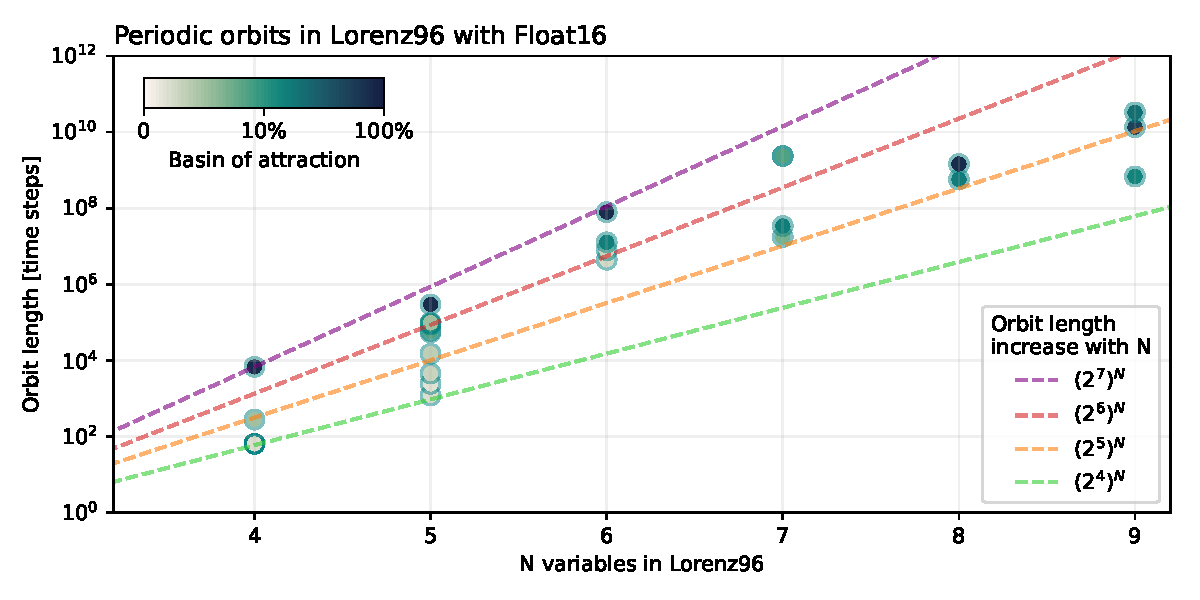
\includegraphics[width=1\textwidth]{Figures/orbits/L96_orbits.pdf}
	\caption{\textbf{Periodic orbits in Lorenz96 simulated with Float16 and an increasing number of
	variables.} Initial conditions are randomly taken from a spin-up simulation. Size of the basins of
	attraction (shading) correspond to the share of initial conditions that converge to the respective
	periodic orbit. Dashed lines provide an orientation for the exponential increase in orbit lengths
	with the number of variables.}
	\label{fig:L96_orbits}
\end{figure}

In most cases between 4 and 9 variables in the Lorenz 1996 system, the longest orbit is also the one with the largest basin of attraction.
The longer the orbit the larger the occupied state space of possible values the variables $X_i$ can take at a given precision. Consequently,
the assumption is that it is most likely that a given trajectory ends up on the longest orbit. However, we also found a counter examples as, 
the longest orbit with $N=8$ variables is shorter than the longest with $N=7$ variables (Figure \ref{fig:L96_orbits}).

\subsection{More variables instead of higher precision}

The orbit length increases approximately exponentially following a scaling of about $16^N$ to $128^N$  from $N=4$ to $N=9$.
Such an exponential increase translates to about 4 to 7 effective bits of freedom (as $2^4=16, 2^7=128$) for every additional
variable in Lorenz 1996 represented with Float16. However, the computational resources limit the orbit search for larger $N$, making
it hard to constrain this exponential scaling further. Assuming a similar exponential orbit increase holds for larger $N$, extrapolation
of these findings suggests orbit lengths on the order of about $10^{100000}$ for million-variable systems simulated with Float16.
This is far beyond the reach of any computational resources currently available. In that sense, while a simulation of such large
systems would eventually be periodic, a periodic solution will never be reached.

\begin{figure}[tbhp]
	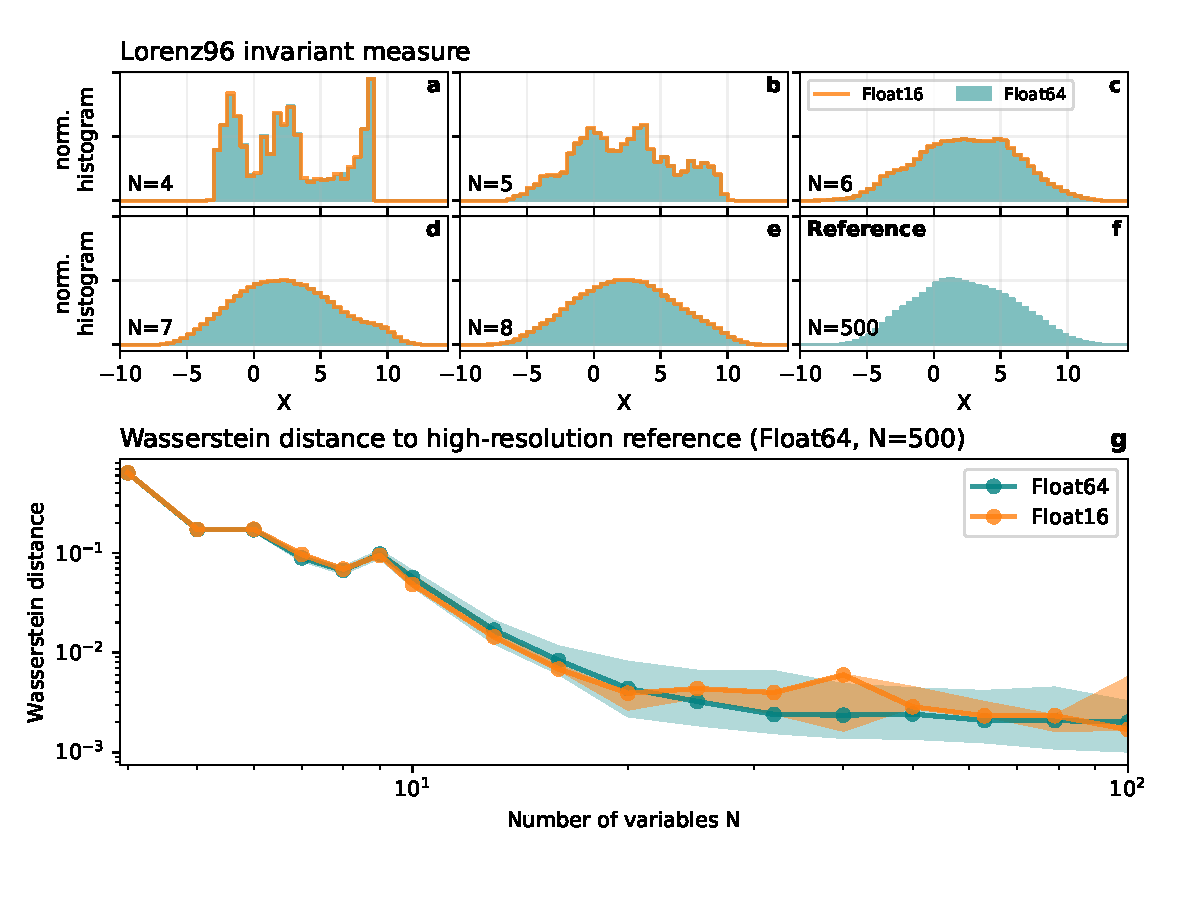
\includegraphics[width=1\textwidth]{Figures/orbits/L96_invmeasures.pdf}
	\caption{\textbf{Improvement of the simulated Lorenz 1996 invariant measure with increasing
	number of variables. a} The invariant measure of Lorenz 1996 simulated with 4 variables. Using
	Float16 or Float64 arithmetic yields a virtually identical invariant measure. b-e as a but with an
	increasing number of variables. f The reference invariant measure obtained from 500 variables
	using Float64 arithmetic. g The Wasserstein distance of the simulated Lorenz 1996 system with
	respect to the reference. Invariant measures are taken from all available variables, which are
	invariant due to periodic boundary conditions and spatially-independent forcing (see Eq. \ref{eq:L96}).
	Shadings in g represent the 5-95\% confidence interval and solid lines the median obtained from
	an ensemble simulation with 51 members starting from slightly perturbed random initial conditions.}
	\label{fig:L96_invmeasures}
\end{figure}

Longer orbits are promising to avoid periodic solutions in low precision, but short periodic orbits do not necessarily misrepresent a
reference invariant measure. We assess the agreement of invariant measures using the Wasserstein distance as before. As a reference
invariant measure $\mu(X_{\op{ref}})$ we integrate the Lorenz 1996 system for 1,000,000 time steps with $N=500$ variables using
Float64 arithmetic. The Wasserstein distance is then $W_1(\mu(X_{\op{ref}}),\mu(X))$ with $X$ representing the $N$ variables from a
Lorenz 1996 simulation using either Float16 or Float64 arithmetic. 

Using only $N=4$ variables in the simulation of Lorenz 1996 yields an invariant measure with little resemblance to the reference (Fig.
\ref{fig:L96_invmeasures}a and e), regardless of the number format. While more variables yield an invariant measure that converges
to the reference, there is virtually no difference whether Float16 or Float64 arithmetic is used (Figure \ref{fig:L96_invmeasures}b-e).
The Wasserstein distance significantly reduces with an increasing number of variables, but not with higher precision. Given a certain
availability of computational resources a better invariant measure is therefore obtained by reducing the precision and reinvesting the
performance gain into more variables.

\section{Discussion}

Non-periodic solutions are an essential property of chaotic dynamical systems. Simulations with deterministic
finite precision numbers, however, always yield periodic orbits. At the high precision of 64-bit floating-point numbers
such orbits are usually negligible due to very long periods. The emerging trend to accelerate simulations with
low-precision numbers, such as 16-bit half precision floats, raises questions on the fidelity of such simulations
of chaotic systems. Here, we revisit the 1-variable chaotic generalised Bernoulli map with floats, posits and
logarithmic fixed-point numbers at various levels of precision using deterministic and stochastic rounding.
The simulations represent the analytical Bernoulli map generally better the higher the precision of the number format.
Stochastic rounding is especially beneficial as it prevents periodic orbits even at low precision. For the simulation
of continuous systems the performance gain from low-precision arithmetic will often be reinvested in higher resolution,
increasing the number of variables. Using the Lorenz 1996 system we provide evidence that the periodic orbit
length increases exponentially with the number of variables. Moreover, invariant measures are often better
approximated, indicating an overall improved simulation, with an increased number of variables than with
increased precision. Extrapolating to complex simulations of natural systems, such as climate models with
millions of variables, periodic orbit lengths are far beyond reach of present-day computers. Periodic orbits from
low-precision simulations are therefore not expected to be problematic for any system larger than the simplest
chaotic systems.
